% figures/growth-loop.tex
% Standalone TikZ: a self-reinforcing growth loop (ch.08).
\documentclass[tikz,border=4pt]{standalone}
\usepackage{tikz}
\usetikzlibrary{arrows.meta,positioning,calc}

\definecolor{loopteal}{HTML}{0E6655}
\definecolor{loopblue}{HTML}{1A5276}

\begin{document}
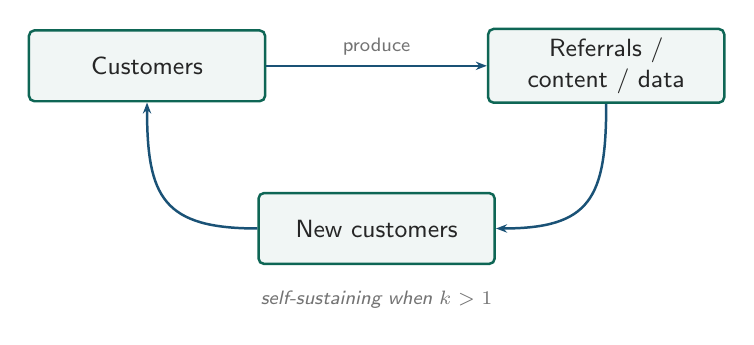
\begin{tikzpicture}[
  node distance=20mm,
  stage/.style={draw=loopteal, line width=0.9pt, rounded corners=2pt, fill=loopteal!6,
                font=\sffamily\small, align=center, minimum width=30mm, minimum height=9mm, text=black!85},
  flow/.style={-{Stealth[length=4pt]}, loopblue, line width=0.9pt},
]
  \node[stage] (cust)  {Customers};
  \node[stage, right=28mm of cust] (out) {Referrals /\\content / data};
  \node[stage, below=16mm of $(cust)!0.5!(out)$] (new) {New customers};

  \draw[flow] (cust.east) -- node[above, font=\scriptsize\sffamily, text=black!55] {produce} (out.west);
  \draw[flow] (out.south) .. controls +(down:12mm) and +(right:12mm) .. (new.east);
  \draw[flow] (new.west) .. controls +(left:12mm) and +(down:12mm) .. (cust.south);

  \node[font=\sffamily\itshape\scriptsize, text=black!55, below=2mm of new]
    {self-sustaining when $k>1$};
\end{tikzpicture}
\end{document}
